
%%%%%%%%%%%%%%%%%%%%%%%%%%%%%%%%%%%%%%%%%%%%%%%%%%%%%%%%%%%%%%%%%%%%%
%% This is a (brief) model paper using the achemso class
%% The document class accepts keyval options, which should include
%% the target journal and optionally the manuscript type.
%%%%%%%%%%%%%%%%%%%%%%%%%%%%%%%%%%%%%%%%%%%%%%%%%%%%%%%%%%%%%%%%%%%%%


\documentclass[journal=jacsat,manuscript=article]{achemso}
\setkeys{acs}{articletitle = true} % show titles in bibliography
%\documentclass[prb,11pt]{revtex4-1}
%\usepackage[sort&compress,numbers,super]{natbib} 
%\usepackage{achemso} 
\SectionNumbersOn 
\usepackage{wrapfig}
\usepackage{xargs}                      % Use more than one optional parameter in a new commands
\usepackage[pdftex,dvipsnames]{xcolor}  % Coloured text etc.
% 
\usepackage[colorinlistoftodos,prependcaption,textsize=tiny]{todonotes}
\newcommandx{\unsure}[2][1=]{\todo[linecolor=red,backgroundcolor=red!25,bordercolor=red,#1]{#2}}
\newcommandx{\change}[2][1=]{\todo[linecolor=OliveGreen,backgroundcolor=OliveGreen!25,bordercolor=OliveGreen,#1]{#2}}
\usepackage{amsfonts}
\usepackage{epigraph}
\setlength{\epigraphwidth}{0.7\textwidth}
%%%%%%%%%%%%%%%%%%%%%%%%%%%%%%%%%%%%%%%%%%%%%%%%%%%%%%%%%%%%%%%%%%%%%
%% Place any additional packages needed here.  Only include packages
%% which are essential, to avoid problems later. Do NOT use any
%% packages which require e-TeX (for example etoolbox): the e-TeX
%% extensions are not currently available on the ACS conversion
%% servers.
%%%%%%%%%%%%%%%%%%%%%%%%%%%%%%%%%%%%%%%%%%%%%%%%%%%%%%%%%%%%%%%%%%%%%
\usepackage[version=3]{mhchem} % Formula subscripts using \ce{}
\usepackage[T1]{fontenc}       % Use modern font encodings
\usepackage{subfig}
\usepackage{url}
\usepackage{xr} % external referecnes
\externaldocument{SI}
\renewcommand{\thepage}{S\arabic{page}}  
\renewcommand{\thesection}{S\arabic{section}}   
\renewcommand{\thetable}{S\arabic{table}}   
\renewcommand{\thefigure}{S\arabic{figure}}
\renewcommand{\theequation}{S\arabic{equation}}
\usepackage{xr} % external referecnes
\externaldocument{latent_space_of_cages}
\usepackage{natbib} 

% so S2.1
\usepackage{chngcntr}
\counterwithin{figure}{section}

% to prevent counter too large in subfigure
\usepackage{alphalph}
\renewcommand*{\thesubfigure}{%
\alphalph{\value{subfigure}}%
}%
%%%%%%%%%%%%%%%%%%%%%%%%%%%%%%%%%%%%%%%%%%%%%%%%%%%%%%%%%%%%%%%%%%%%%
%% If issues arise when submitting your manuscript, you may want to
%% un-comment the next line.  This provides information on the
%% version of every file you have used.
%%%%%%%%%%%%%%%%%%%%%%%%%%%%%%%%%%%%%%%%%%%%%%%%%%%%%%%%%%%%%%%%%%%%%
%%\listfiles

%%%%%%%%%%%%%%%%%%%%%%%%%%%%%%%%%%%%%%%%%%%%%%%%%%%%%%%%%%%%%%%%%%%%%
%% Place any additional macros here.  Please use \newcommand* where
%% possible, and avoid layout-changing macros (which are not used
%% when typesetting).
%%%%%%%%%%%%%%%%%%%%%%%%%%%%%%%%%%%%%%%%%%%%%%%%%%%%%%%%%%%%%%%%%%%%%
\newcommand*\mycommand[1]{\texttt{\emph{#1}}}

%%%%%%%%%%%%%%%%%%%%%%%%%%%%%%%%%%%%%%%%%%%%%%%%%%%%%%%%%%%%%%%%%%%%%
%% Meta-data block
%% ---------------
%% Each author should be given as a separate \author command.
%%
%% Corresponding authors should have an e-mail given after the author
%% name as an \email command. Phone and fax numbers can be given
%% using \phone and \fax, respectively; this information is optional.
%%
%% The affiliation of authors is given after the authors; each
%% \affiliation command applies to all preceding authors not already
%% assigned an affiliation.
%%
%% The affiliation takes an option argument for the short name.  This
%% will typically be something like "University of Somewhere".
%%
%% The \altaffiliation macro should be used for new address, etc.
%% On the other hand, \alsoaffiliation is used on a per author basis
%% when authors are associated with multiple institutions.
%%%%%%%%%%%%%%%%%%%%%%%%%%%%%%%%%%%%%%%%%%%%%%%%%%%%%%%%%%%%%%%%%%%%%
\author{Arni Sturluson}
\affiliation[Oregon State University]
{School of Chemical, Biological, and Environmental Engineering. Corvallis, OR, USA.}
\author{Melanie T. Huynh}
\affiliation[Oregon State University]
{School of Chemical, Biological, and Environmental Engineering. Corvallis, OR, USA.}
\author{Arthur H. P. York}
\affiliation[Oregon State University]
{School of Chemical, Biological, and Environmental Engineering. Corvallis, OR, USA.}
\author{Cory M. Simon}
%\altaffiliation{A shared footnote}
\email{Cory.Simon@oregonstate.edu}
\affiliation[Oregon State University]
{School of Chemical, Biological, and Environmental Engineering. Corvallis, OR, USA.}
%\altaffiliation{A shared footnote}
%\email{Cory.Simon@oregonstate.edu}
%\affiliation[Oregon State University]
%{School of Chemical, Biological, and Environmental Engineering. Corvallis, OR, USA.}
%\author{Carlo Carraro}
%\affiliation[University of California, Berkeley]
%{Department of Chemical and Biomolecular Engineering. Berkeley, CA, USA.}
%\altaffiliation{Current address: Some other place, Othert\"own,
%Germany}
%\author{I. Ken Groupleader}
%\altaffiliation{A shared footnote}
%\email{i.k.groupleader@unknown.uu}
%\phone{+123 (0)123 4445556}
%\fax{+123 (0)123 4445557}
%\affiliation[Unknown University]
%{Department of Chemistry, Unknown University, Unknown Town}
%\alsoaffiliation[Second University]
%{Department of Chemistry, Second University, Nearby Town}
%\author{Susanne K. Laborator}

%\affiliation[BigPharma]
%{Lead Discovery, BigPharma, Big Town, USA}
%\author{Kay T. Finally}



%%%%%%%%%%%%%%%%%%%%%%%%%%%%%%%%%%%%%%%%%%%%%%%%%%%%%%%%%%%%%%%%%%%%%
%% The document title should be given as usual. Some journals require
%% a running title from the author: this should be supplied as an
%% optional argument to \title.
%%%%%%%%%%%%%%%%%%%%%%%%%%%%%%%%%%%%%%%%%%%%%%%%%%%%%%%%%%%%%%%%%%%%%
\title[SI: Latent Space of Porous Cages]
  {Supporting Information for: Eigencages: {\color{red} Learning a latent space of porous cage molecules}}

%%%%%%%%%%%%%%%%%%%%%%%%%%%%%%%%%%%%%%%%%%%%%%%%%%%%%%%%%%%%%%%%%%%%%
%% Some journals require a list of abbreviations or keywords to be
%% supplied. These should be set up here, and will be printed after
%% the title and author information, if needed.
%%%%%%%%%%%%%%%%%%%%%%%%%%%%%%%%%%%%%%%%%%%%%%%%%%%%%%%%%%%%%%%%%%%%%
\abbreviations{IR,NMR,UV}
\keywords{American Chemical Society, \LaTeX}
\newcommand{\angstrom}{\mbox{\normalfont\AA}}

%%%%%%%%%%%%%%%%%%%%%%%%%%%%%%%%%%%%%%%%%%%%%%%%%%%%%%%%%%%%%%%%%%%%%
%% The manuscript does not need to include \maketitle, which is
%% executed automatically.
%%%%%%%%%%%%%%%%%%%%%%%%%%%%%%%%%%%%%%%%%%%%%%%%%%%%%%%%%%%%%%%%%%%%%
\begin{document}

%%%%%%%%%%%%%%%%%%%%%%%%%%%%%%%%%%%%%%%%%%%%%%%%%%%%%%%%%%%%%%%%%%%%%
%% The "tocentry" environment can be used to create an entry for the
%% graphical table of contents. It is given here as some journals
%% require that it is printed as part of the abstract page. It will
%% be automatically moved as appropriate.
%%%%%%%%%%%%%%%%%%%%%%%%%%%%%%%%%%%%%%%%%%%%%%%%%%%%%%%%%%%%%%%%%%%%%
%\begin{tocentry}
%
%Some journals require a graphical entry for the Table of Contents.
%This should be laid out ``print ready'' so that the sizing of the
%text is correct.
%
%Inside the \texttt{tocentry} environment, the font used is Helvetica
%8\,pt, as required by \emph{Journal of the American Chemical
%Society}.
%
%The surrounding frame is 9\,cm by 3.5\,cm, which is the maximum
%permitted for  \emph{Journal of the American Chemical Society}
%graphical table of content entries. The box will not resize if the
%content is too big: instead it will overflow the edge of the box.
%
%This box and the associated title will always be printed on a
%separate page at the end of the document.
%
%\end{tocentry}

%%%%%%%%%%%%%%%%%%%%%%%%%%%%%%%%%%%%%%%%%%%%%%%%%%%%%%%%%%%%%%%%%%%%%
%% The abstract environment will automatically gobble the contents
%% if an abstract is not used by the target journal.
%%%%%%%%%%%%%%%%%%%%%%%%%%%%%%%%%%%%%%%%%%%%%%%%%%%%%%%%%%%%%%%%%%%%%
%\begin{abstract}
%We use statistical thermodynamics to answer a simple question: what happens when an adsorbent is allowed to exchange gas with a rubber balloon? Richard Feynman described rubber as 'molecular spaghetti'. A statistical mechanical treatment of this molecular view of rubber captures the relationship between the pressure of gas in a rubber balloon and its radius. As a consequence of the non-monotonicity of this relationship, a gas-adsorbent-balloon system presents multi- and in-stabilities. In contrast, we show that two different adsorbents allowed to exchange gas cannot exhibit multi-stability.
%\end{abstract}

%%%%%%%%%%%%%%%%%%%%%%%%%%%%%%%%%%%%%%%%%%%%%%%%%%%%%%%%%%%%%%%%%%%%%
%% Start the main part of the manuscript here.
%%%%%%%%%%%%%%%%%%%%%%%%%%%%%%%%%%%%%%%%%%%%%%%%%%%%%%%%%%%%%%%%%%%%%
\section{Distribution of cage molecule and cavity diameters}

\begin{figure}
\centering
	\includegraphics[width=0.65\columnwidth]{../pywindow_descriptors_distn.png}
	\caption{The distribution of cage molecule diameters (red) and cage cavity diameters (blue) among the 74 cages analyzed in this work. These diameters were computed with \texttt{pywindow}. \cite{miklitz2018pywindow}.
	} \label{fig:pywindow_descriptors_distn}
\end{figure}

\newpage
\clearpage

\section{Aligning the cages before scanning for void space} 
\label{sec:alignment_details}
We compute the $3\times 3$ symmetric moment of inertia matrix $\mathbf{I}$ of the cage, defined relative to the center of mass, and find its eigendecomposition $\mathbf{I}=\mathbf{W}\mathbf{\Lambda}\mathbf{W^T}$, with the eigenvalues arranged in a non-increasing order down the diagonal matrix $\mathbf{\Lambda}$ and the orthonormal eigenvectors in the columns of $\mathbf{W}$. {\color{red} The eigenvectors of the matrix $\mathbf{I}$ are the principal axes of inertia, and the associated eigenvalues are the moments of inertia with respect to those axes.} Then, we transform the coordinates of the centered cage by left-multiplying by the rotation matrix $\mathbf{W^T}$. The rotated cage then possesses a diagonal moment of inertia matrix with the moments of inertia arranged in a non-increasing order down the diagonal.

{\color{red}
\subsection{Degenerate principal axes of inertia}
Molecules that exhibit symmetry can possess degenerate moments and principal axes of inertia. As an example, consider sulfur trioxide (SO$_3$), a trigonal planar molecule, shown in Fig.~\ref{fig:SO3}. Its moment of inertia matrix $\mathbf{I}$, with Cartesian directions defined in Fig.~\ref{fig:SO3} and the sulfur atom at the origin, is:
\begin{equation}
\mathbf{I} = m_{\text{O}} \ell_{S-O}^2
  \begin{bmatrix}
    3/2 & 0 & 0 \\
    0 & 3/2 & 0 \\
    0 & 0 & 3
  \end{bmatrix}, \label{eq:I_SO3}
\end{equation} where $m_{\text{O}}$ is the mass of an oxygen atom and $\ell_{S-O}$ is the sulfur-oxygen bond length. The eigenvalues of the moment of inertia matrix $\mathbf{I}$ are 3/2, 3/2, and 3 times $m_{\text{O}} \ell_{S-O}^2$. The eigenvector (unique if unit norm enforced) associated with the largest eigenvalue, $3 m_{\text{O}} \ell_{S-O}^2$, is $[0, 0, 1]$, indicating that the principal axis of inertia with the largest moment of inertia is pointing into the page with respect to Fig.~\ref{fig:SO3}. The remaining two principal axes of inertia must be orthogonal to $[0, 0, 1]$ and thus lay in the $x$-$y$ plane. The moments of inertia about the remaining two principal axes of inertia, however, are equal, as the remaining eigenvalues 3/2, 3/2 times $m_{\text{O}} \ell_{S-O}^2$ are degenerate. In fact, \emph{any} vector laying in the $x$-$y$ plane are eigenvectors of the matrix $\mathbf{I}$ in eqn.~\ref{eq:I_SO3} associated with eigenvalue $3m_{\text{O}} \ell_{S-O}^2/2$. This mathematically indicates that the two remaining principal axes of inertia for SO$_3$ are not unique.

\begin{figure}
\centering
%	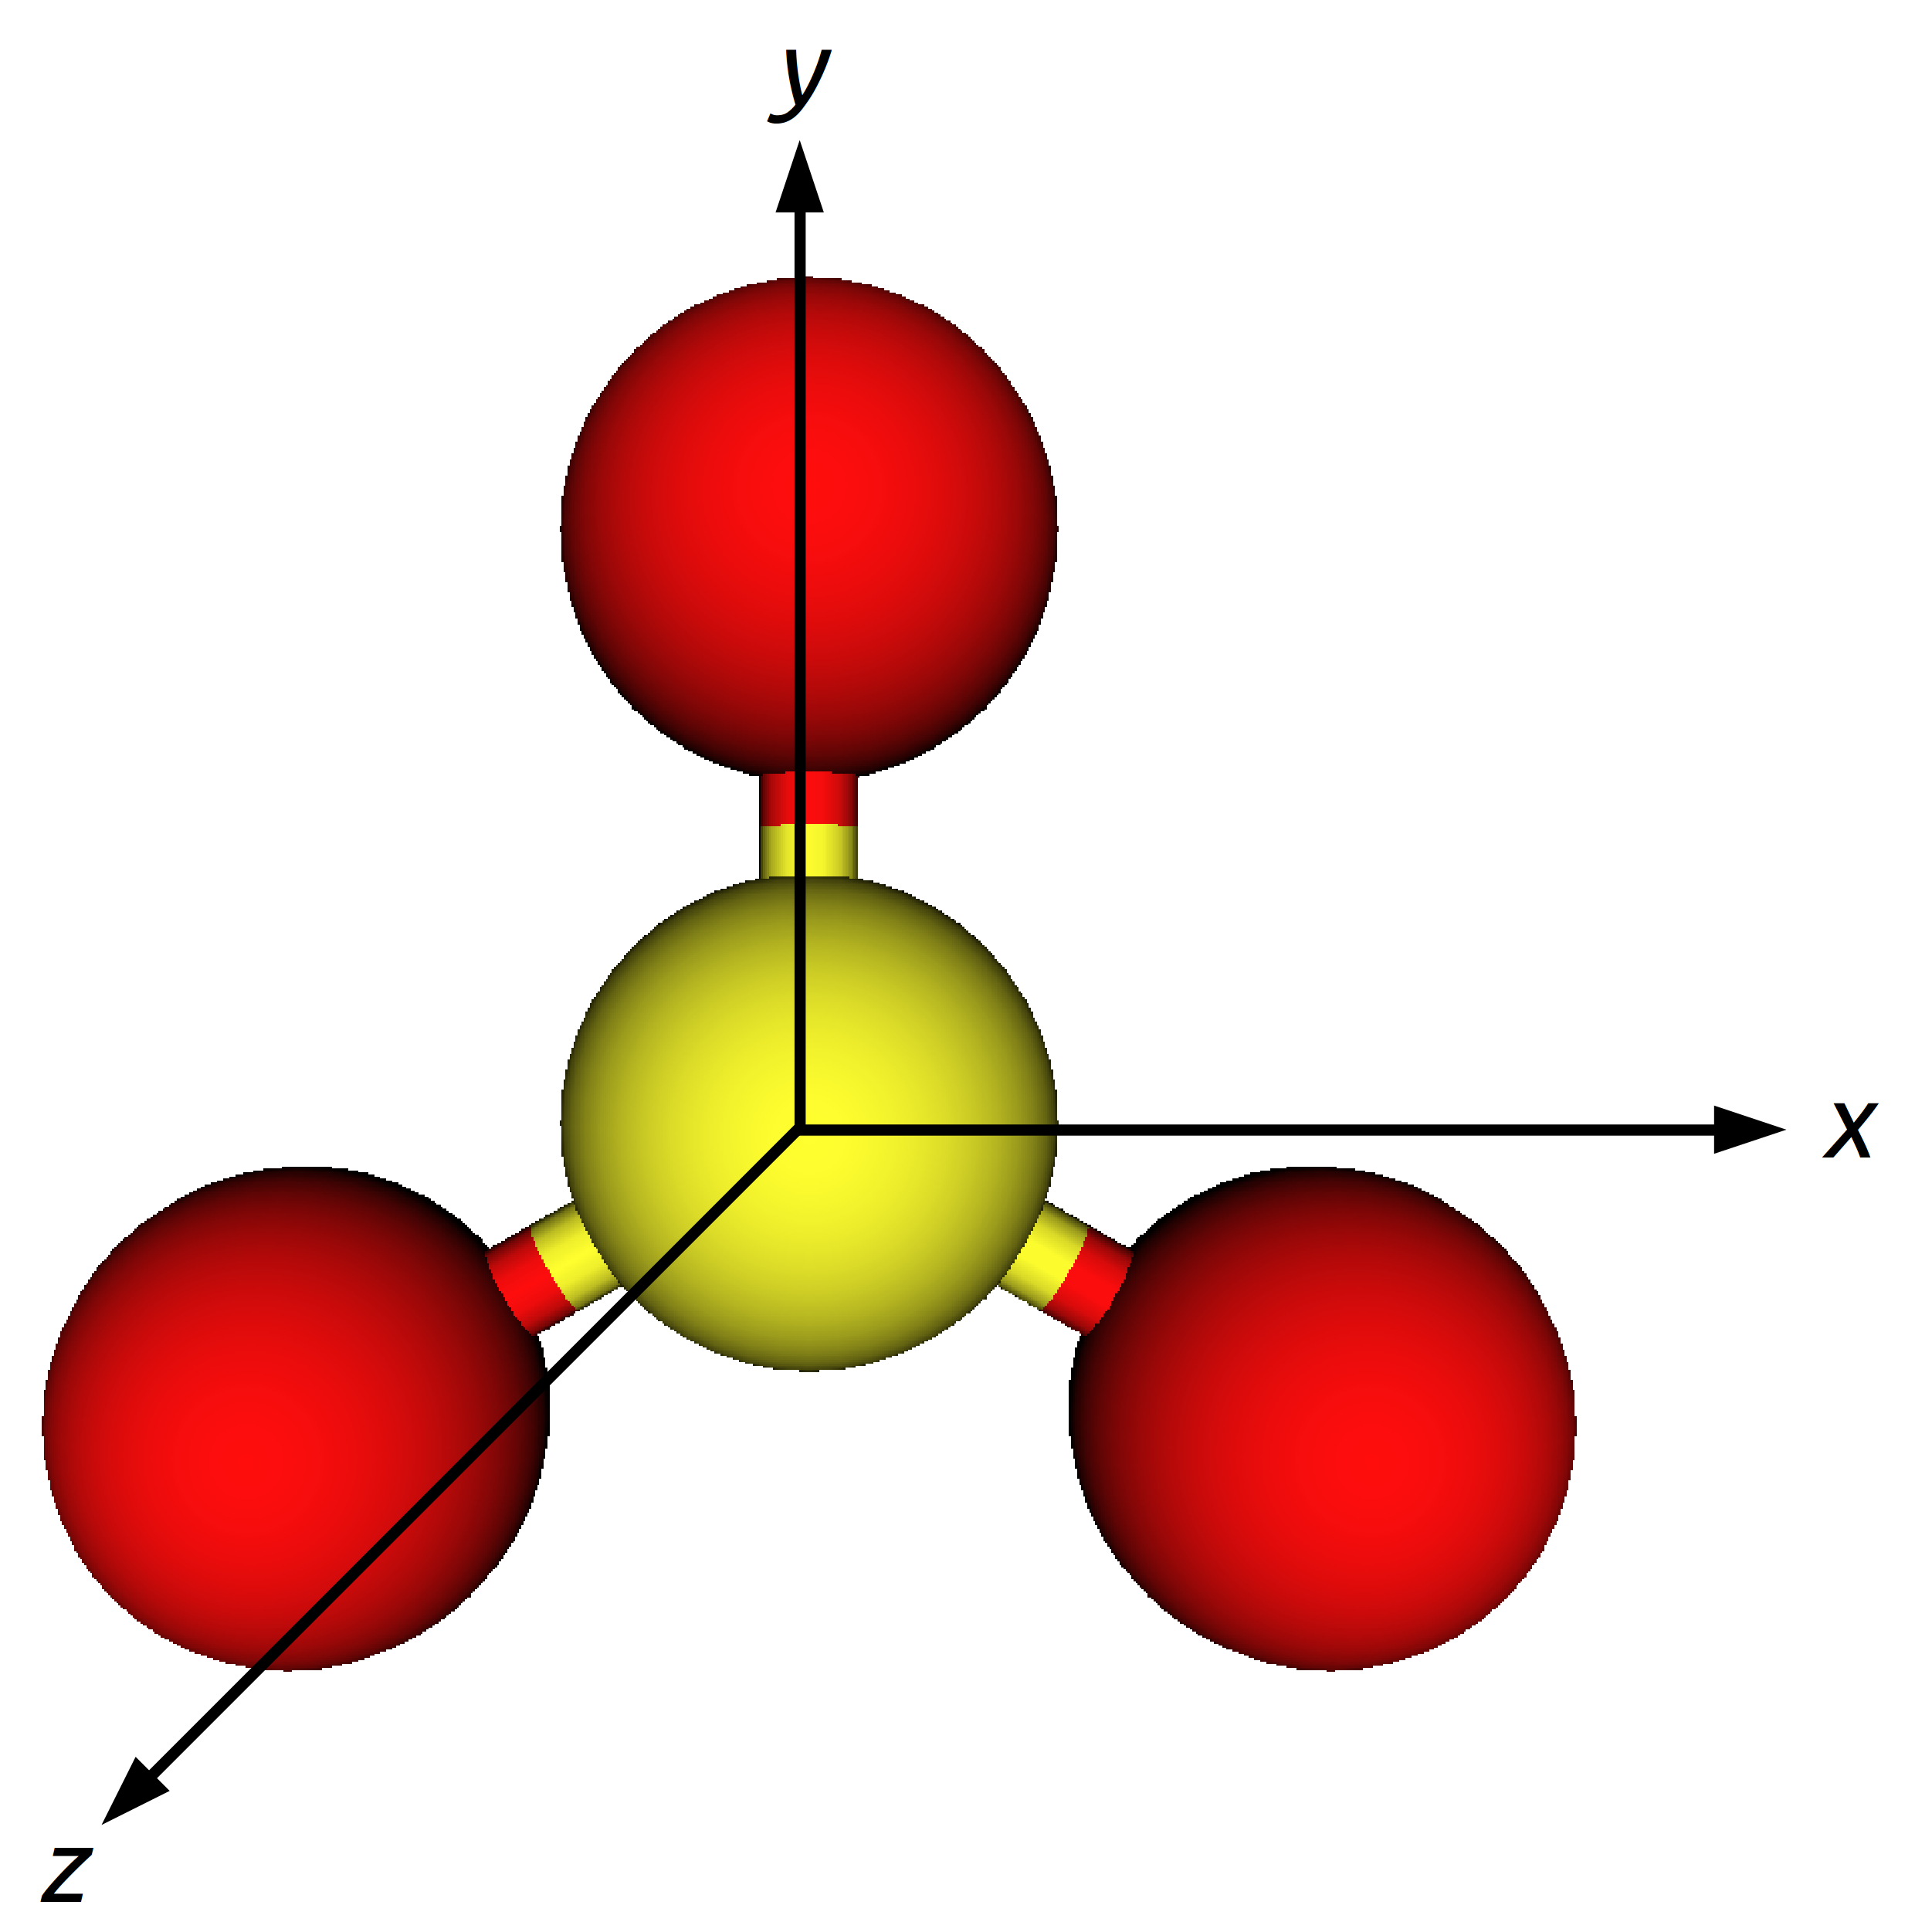
\includegraphics[width=0.3\columnwidth]{../principal_axes_rotation_failure/SO3_axes_marked.png}
	\caption{{\color{red} Sulfur trioxide (SO$_3$) is a trigonal planar molecule with degenerate principal axes of inertia in the x-y plane.
	}% color red end
	} \label{fig:SO3}
\end{figure}

As a consequence, the principal axes of inertia for a symmetric molecule such as SO$_3$ do not provide a means to uniquely align the molecule. Thus, e.g. to compare SO$_3$ with respect to a molecule exhibiting the same trigonal planar symmetry, such as boron trifluoride BF$_3$, the principal axes of inertia cannot be used to align the two molecules along their bonds (aside from the principal axes of inertia associated with the largest moment of inertia, $[0 0 1]$ in Fig.~\ref{fig:SO3}). With regards to its rotational dynamics, SO$_3$ behaves as a uniform disk \cite{peraire2008lecture}.

Several cage molecules exhibit a high degree of rotational symmetry, so as to behave akin to SO$_3$, where the principal axes of inertia are not unique and thus cannot be used to consistently align them. For example, the three moments of inertia of CC1 (15869.8, 15869.6, 15869.4 amu-$\angstrom^2$) and of CC3 (32767.1, 32766.9, 32766.6 amu-$\angstrom^2$) are nearly equal, indicating that the rotational dynamics of CC1 and CC3 are akin to a sphere; therefore, using the principal axes of inertial to align CC1 and CC3 (i) theoretically will not provide a unique manner in which to align them and (ii) will be extremely sensitive to small perturbations in the structure. Note that CC3 and CC1 differ only in the vertices external to the cavity, but, as Fig.~\ref{fig:misaligned} shows, CC1 and CC3 are aligned irrationally on the basis of their computed principal axes of inertia due to the [near-]degeneracy of their axes of inertia. Another example that is highly related to the SO$_3$ example in Fig.~\ref{fig:SO3} are B6 and B8, also shown in Fig.~\ref{fig:misaligned}. Here, small differences in the three propeller-blade-like moieties that protrude from B6 and B8 result in significantly inconsistent alignments for comparing B6 and B8. B6 and B8 much resemble the SO$_3$ example in Fig.~\ref{fig:SO3}, as two principal axes of inertia are nearly degenerate and thus the principal axes in that plane (the plane of the page in Fig.~\ref{fig:allcagesdetailed}) are very sensitive to small perturbations in the structure.

\begin{figure}
\centering
	\subfloat[][CC3]{\includegraphics[width=0.45\columnwidth]{../all_cages/CC3_final_alignment.png}}
	\subfloat[][CC1]{\includegraphics[width=0.45\columnwidth]{../all_cages/CC1_final_alignment.png}} \qquad
		\subfloat[][B6]{\includegraphics[width=0.45\columnwidth]{../all_cages/B6_final_alignment.png}}
	\subfloat[][B8]{\includegraphics[width=0.45\columnwidth]{../all_cages/B8_final_alignment.png}}
	\caption{{\color{red} Cases where the computed principal axes of inertia do not provide reasonable alignments of cages. (a, b) The rotational dynamics of CC1 and CC3 are akin to a sphere; the three moments of inertia for each CC1 and CC3 are computed to be approximately equal (CC1: 15869.8, 15869.6, 15869.4 amu-$\angstrom^2$; CC3: 32767.1, 32766.9, 32766.6 amu-$\angstrom^2$). Shown are the two cages aligned with their computed principal axes of inertia. Despite differing only in the their vertices at the periphery of the cage, the two molecules are aligned inconsistently/irrationally. (c, d) Shown are cages B6 and B8 aligned with their principal axes of inertia. B6 and B8 have two nearly degenerate axes of inertia (B6: 39371.2, 29141.2, 28881.8 amu-$\angstrom^2$; B8: 27874.4, 23253.6, 23190.7 amu-$\angstrom^2$). As a result, despite only subtle differences in the three propeller-blade-like moieties that protrude from their cores, the molecules are not aligned consistently.
	}% color red end
	} \label{fig:misaligned}
\end{figure}

Therefore, the principle axes of inertia are in many cases insufficient to determine an alignment of a porous cage molecule that is unique and robust to small differences. Fig.~\ref{fig:moments_of_inertia} displays the three moments of inertia with respect to the principal axes of inertia for each centered cage, normalized by the largest moment of inertia. Cages with uncolored bars, such as MC1 and MC4, display a significant difference between the three moments of inertia; therefore for these cages, the  principal axes of rotation are a good way to consistently align these cages with similar cages. On the other hand, cages that have colored bars, such as CC1 and CC3, possess moments of inertia that are quite close to one another. We define consecutive moments of inertia to be \emph{practically degenerate} (and color them in Fig.~\ref{fig:moments_of_inertia}) when placing a single carbon atom at the periphery of the molecule in the direction of a principal axis changes the ranking of the principal axes of inertia. i.e., if the moments of inertia differ by less than $12 r^2$ amu-$\angstrom$, where $r$ is the radius of the cage molecule, we decide that the principal axes of inertia do not provide a reasonable method to consistently align the cage with similar cages because small differences can drastically change the orientations.

\begin{figure}
\centering
\includegraphics[width=\columnwidth]{../moments_of_inertia.pdf}
	\caption{{\color{red} Moments of inertia of the cages about their principal axes of rotation. Each panel corresponds to a different cage. The three bars are the three moments of inertia about the principal axes of rotation (the eigenvalues $\lambda_i$ of the moment of inertia matrix), normalized by the largest moment of inertia. Bars are colored if two consecutive moments of inertia differ by less than $12 r^2$ amu-$\angstrom$, where $r$ is the radius of the cage molecule. Red: all moments of inertia are practically degenerate; blue, green: the first two and last two, respectively, moments of inertia are practically degenerate. For cages with colored bars, the principal axes of inertia do not provide a reasonable method to consistently align the cage with similar cages because small differences can drastically change the orientation.
	}% color red end
	} \label{fig:moments_of_inertia}
\end{figure}

We conclude that the set of cages with practically degenerate principal axes of inertia in Fig.~\ref{fig:moments_of_inertia} cannot be aligned using their principal axes of inertia because these alignments will not be robust to small changes in the structure.


} % end color red

\newpage

\section{The data matrix $\mathbf{A}$}

\begin{figure}
\centering
	\includegraphics[width=\columnwidth]{../data_matrix_viz.png}
	\caption{An attempt at visualizing the structure of the $c \times g^3$ data matrix $\mathbf{A}$. The color depicts the magnitude of the entry of the matrix. This is an ``attempt'' because $g^3>>c$, so the data matrix $\mathbf{A}$ is wide and difficult to visualize without a longer page. Zoom in to see some structure. We remark that 10879/15625 of the columns (representing pixels in the cage void space images) are all zeros.
	} \label{fig:data_matrix}
\end{figure}

\newpage
\clearpage

\section{The singular values of $\mathbf{A}$}

\begin{figure}
\centering
	\includegraphics[width=0.65\columnwidth]{../distn_of_svs.png}
	\caption{The distribution of the set of singular values $\sigma_1,\sigma_2, ..., \sigma_{74}$ of $\mathbf{A}$.
	} \label{fig:distn_of_svs}
\end{figure}

\newpage
\clearpage

\section{Relative error from approximating $\mathbf{A}$ as $\mathbf{A}_\nu$}

\begin{figure}
\centering
	\includegraphics[width=0.65\columnwidth]{../relative_err_with_svs.png}
	\caption{The relative error in approximating the data matrix $\mathbf{A}$ with a lower-rank-$\nu$ approximant $\mathbf{A}_\nu$ given in eqn.~\ref{eq:Anu}. The formula for the relative error as a function of $\nu$, related to the singular values of $\mathbf{A}$, is given in eqn.~\ref{eq:relative_error}.
	} \label{fig:relative_err_with_svs}
\end{figure}

\newpage
\clearpage

\section{Highlighting remaining clusters in latent cage space}

\begin{figure}[h!]
\centering
	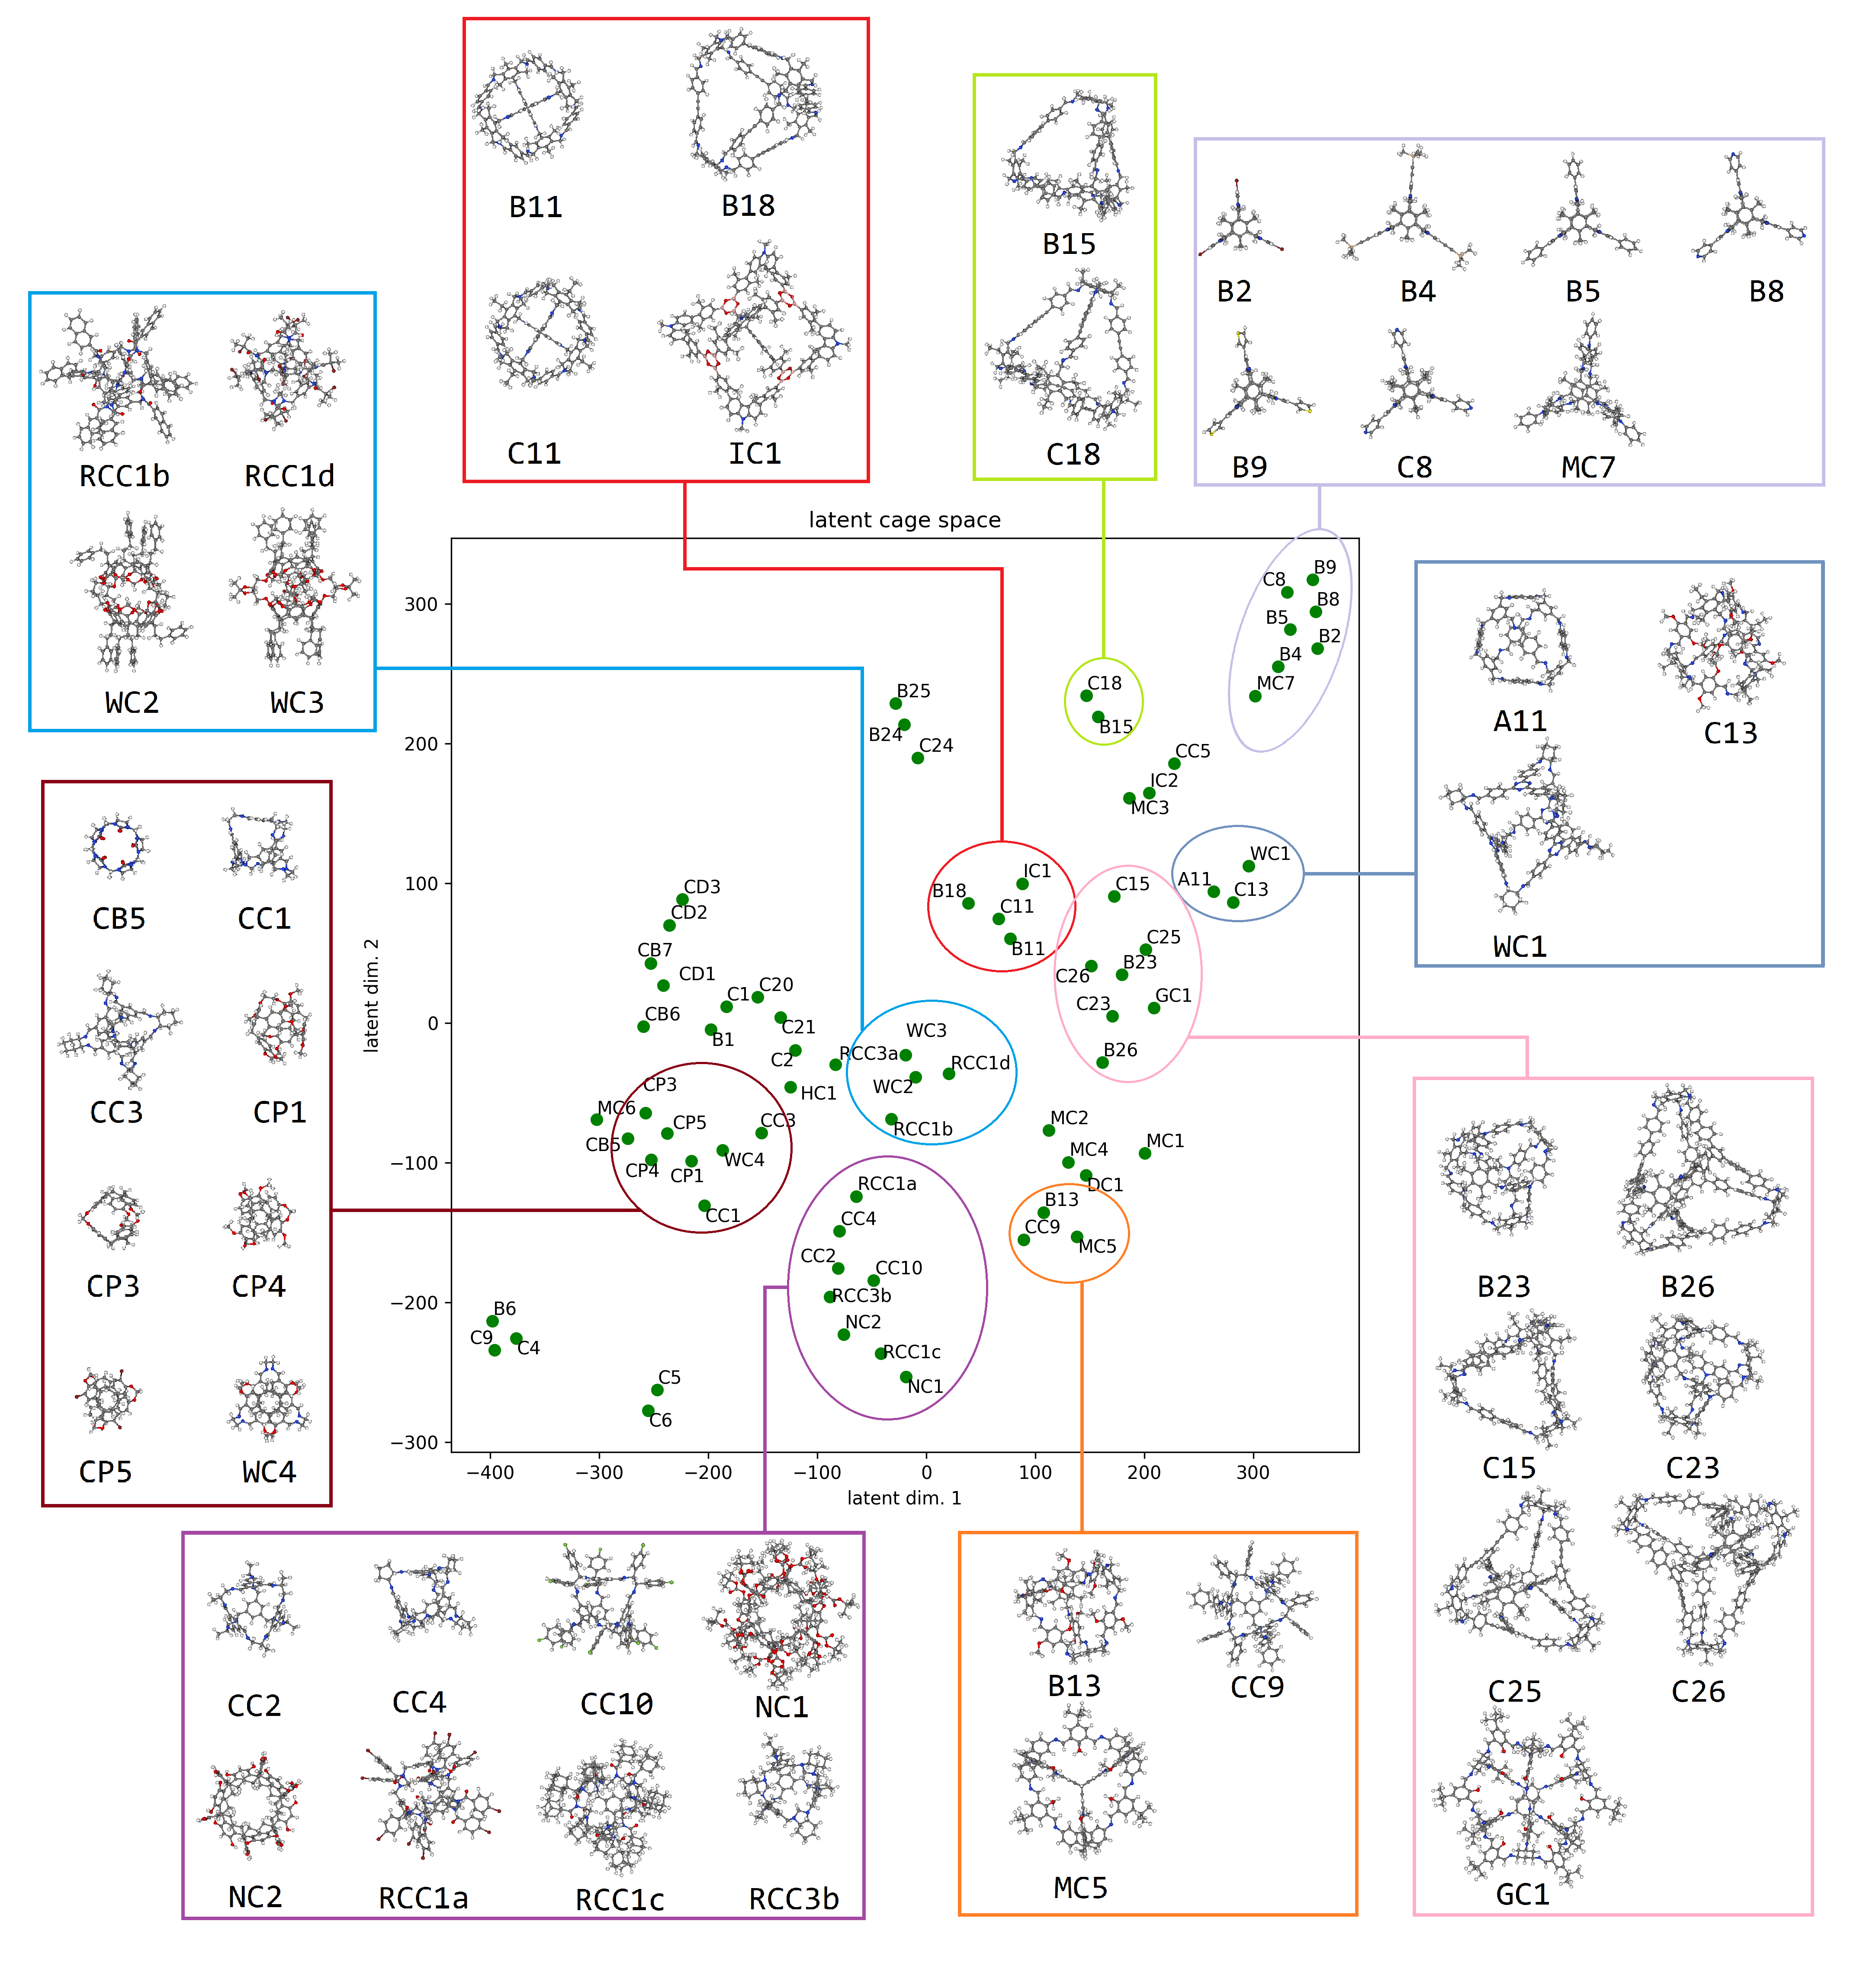
\includegraphics[width=0.9\columnwidth]{../latent_cage_space_2D_marked_SI.png}
	\caption{The latent space of cages $\mathbf{U}_\nu \mathbf{\Sigma}_\nu$ embedded into 2D by t-SNE \cite{maaten2008visualizing,wattenberg2016how}. Salient clusters are highlighted. See Fig.~\ref{fig:latent_space} for the remaining clusters.
	} \label{fig:latent_space2}
\end{figure}


\newpage
\clearpage


\section{Henry coefficient calculations} \label{sec:henrydetails} We describe more details here of the Henry coefficient calculations used to obtain the data in Fig.~\ref{fig:latent_space_S_Xe_Kr}. We model the energetics of the interaction of a gas atom (Xe, Kr, He) with the atoms of the cage as pairwise additive and with 12-6 Lennard-Jones potentials. The $\epsilon_i$ and $\sigma_i$ parameters of the Lennard-Jones potentials for atom $i$- atom $i$ interactions are taken from the Universal Force Field \cite{rappe1992uff} (cutoff radius 14~$\angstrom$). Geometric mixing rules are applied for cross-interactions. 

We placed an isolated cage molecule in an empty simulation box and took it as rigid. If $\mathbf{x} \in \mathbb{R}^3$ is the position of a gas atom in the simulation box, the molecular model described above gives us the potential energy of the gas molecule, $U(\mathbf{x})$.

Consider the isolated porous cage molecule immersed in a bath of gas; the simulation box is drawn around the porous cage molecule. Henry's law models the density of gas in the simulation box at thermodynamic equilibrium, $\rho $, as $\rho=K P$, with $K$ the Henry coefficient and $P$ the pressure of the gas. Henry's law is valid only at low surface coverage.

The Henry coefficient of a gas in the simulation box including the isolated cage molecule is given as:
\begin{equation}
K = \beta \frac{1}{|\Omega|} \int_\Omega e^{-\beta U(\mathbf{x})} d\mathbf{x},
\label{eq:K}
\end{equation} where $\beta= (k_B T)^{-1}$ is the thermodynamic beta ($T$ temperature, $k_B$ Boltzmann constant) and the integral is over the simulation box $\Omega$ (which has volume $|\Omega|$). Note that if $U(\mathbf{x})=0$, Henry's law recovers the ideal gas law $\rho = \beta P$, where $|\Omega|$ is the volume of the simulation box.

We computed the average in eqn.~\ref{eq:K} via Monte Carlo integration, i.e. Widom particle insertions \cite{frenkel2001understanding}, using 1000 Monte Carlo insertions per volume ($\angstrom^3$) of the simulation box. We used \texttt{PorousMaterials.jl} v0.1.1 \cite{PorousMaterialsJL} to compute the Henry coefficient.

\subsection{Comparing to experimental data}
By considering only an isolated cage molecule in a simulation box, as opposed to many cage molecules packed together to form a solid, we account for only the influence of the intrinsic porosity to the cage molecule on the adsorption. This is an approximation, as we are neglecting the influence of the extrinsic porosity that arises from how the cage molecules pack together to form a bulk solid. When the cage molecules pack together, the adsorption sites on the exterior of the molecule or at the cage windows can be modified depending on how the cage molecules pack together. However, when the interior of the cage molecule is the dominant adsorption site in the bulk solid, this approach may be a viable method to predict the Henry coefficient of a bulk porous cage solid.

To evaluate our crude method of considering an isolated cage molecule, Fig.~\ref{fig:expt_sim_compare} compares experimentally measured xenon and krypton adsorption isotherms in noria \cite{patil2016noria} (NC2) and CC3 \cite{chen2014separation} to the resulting Henry's law with the Henry coefficient obtained from our simulations. Fig.~\ref{fig:expt_sim_compare} shows this method yields a very good prediction of experimental Xe and Kr Henry coefficients in noria \cite{patil2016noria} (NC2), but underestimates the Henry coefficients in CC3 \cite{chen2014separation}. See Patil et al. \cite{patil2016noria} for more discussion.

\begin{figure}
\centering
	\includegraphics[width=0.4\columnwidth]{../noria_expt_sim_comparison.png}
	\includegraphics[width=0.4\columnwidth]{../CC3_expt_sim_comparison.png}
	\caption{Comparison of experimental xenon and krypton adsorption isotherms at 298 K in noria \cite{patil2016noria} and CC3 \cite{chen2014separation} to the simulated adsorption. Points show experimental data and the lines show Henry's law with the Henry coefficient taken from our simulations. The simulated Henry coefficient of He was subtracted to account for the empty space in the simulation box.
	} \label{fig:expt_sim_compare}
\end{figure}

\newpage
\clearpage

\section{Relationship of latent representation and cage molecule and cavity diameters}
Fig.~\ref{fig:first_component_captures_pore_diameter} shows that the first component of the learned latent representation of a cage is strongly correlated with its cavity diameter. 
Fig.~\ref{fig:cage_space_colored_by_diams_2D} depicts how the 2D embedding (by t-SNE) of the $\nu=23$ dimensional latent representations is correlated with the molecule diameter and cavity diameter of a porous organic cage molecule.

\begin{figure}
\centering
	\includegraphics[width=0.9\columnwidth]{../first_component_captures_pore_diameter.pdf}
	\caption{The first component of the latent representation of a cage is strongly correlated to its cavity diameter. The cavity diameter was computed by \texttt{pywindow} \cite{miklitz2018pywindow}. In the reconstruction of the 3D void space image of a given cage, the first component of the latent representation (in the first column of $\mathbf{U}_\nu \mathbf{\Sigma}_\nu$) is the weight on the first eigencage $\mathbf{v}_1$ in the reconstruction of the 3D void space image via eqn.~\ref{eq:latent_space_view}. That the first eigencage is a good descriptor of pore size is suggested by the radial symmetry of the core of the first eigencage in Fig.~\ref{fig:eigencages} that is added to the approximately radially symmetric average cage $\bar{\mathbf{c}}$ to reconstruct the 3D void space image via eqn.~\ref{eq:latent_space_view}.
	} \label{fig:first_component_captures_pore_diameter}
\end{figure}


\begin{figure}
\centering
	\includegraphics[width=\columnwidth]{../cage_space_colored_by_diams_2D.png}
	\caption{The 2D embedding (by t-SNE) of the learned latent representation of the 3D void space images contained in the rows of $\mathbf{U}_\nu \mathbf{\Sigma}_\nu$. Here, the diameter of points represents molecule diameter; color represents cavity diameter, both computed by \texttt{pywindow} \cite{miklitz2018pywindow}. Note that neighbors in latent space tend to have similar cavity and molecule diameters.
	} \label{fig:cage_space_colored_by_diams_2D}
\end{figure}

\newpage
\clearpage

\section{Relationship of latent representation and number of windows to enter cavity}

\begin{figure}
\centering
	\includegraphics[width=\columnwidth]{../cage_space_colored_by_nb_windows.png}
	\caption{The 2D embedding (by t-SNE) of the learned latent representation of the 3D void space images contained in the rows of $\mathbf{U}_\nu \mathbf{\Sigma}_\nu$. Here, the color represents the number of windows possessed by the cage molecule. The gas molecules enter the cavity of the cage through the windows. The number of windows is computed by \texttt{pywindow} \cite{miklitz2018pywindow}. Note that cages within clusters in latent space have the same number of windows.
	} \label{fig:cage_space_colored_by_nb_windows}
\end{figure}

\newpage
\clearpage


% see viz.ipynb
\section{Visualization of the cage structures}
Larger images of the cages in Fig.~\ref{fig:cages} are shown in Fig.~\ref{fig:allcagesdetailed}.
\captionsetup[subfigure]{labelformat=empty} % get rid of a b c d
\begin{figure}[!h]
\centering
\subfloat[A11]{\includegraphics[width=0.25\columnwidth]{../all_cages/A11_final_alignment.png}}
\subfloat[B11]{\includegraphics[width=0.25\columnwidth]{../all_cages/B11_final_alignment.png}}
\subfloat[B13]{\includegraphics[width=0.25\columnwidth]{../all_cages/B13_final_alignment.png}}
\qquad
\subfloat[B15]{\includegraphics[width=0.25\columnwidth]{../all_cages/B15_final_alignment.png}}
\subfloat[B18]{\includegraphics[width=0.25\columnwidth]{../all_cages/B18_final_alignment.png}}
\subfloat[B1]{\includegraphics[width=0.25\columnwidth]{../all_cages/B1_final_alignment.png}}
\qquad
\subfloat[B23]{\includegraphics[width=0.25\columnwidth]{../all_cages/B23_final_alignment.png}}
\subfloat[B24]{\includegraphics[width=0.25\columnwidth]{../all_cages/B24_final_alignment.png}}
\subfloat[B25]{\includegraphics[width=0.25\columnwidth]{../all_cages/B25_final_alignment.png}}
\qquad
\subfloat[B26]{\includegraphics[width=0.25\columnwidth]{../all_cages/B26_final_alignment.png}}
\subfloat[B2]{\includegraphics[width=0.25\columnwidth]{../all_cages/B2_final_alignment.png}}
\subfloat[B4]{\includegraphics[width=0.25\columnwidth]{../all_cages/B4_final_alignment.png}}
\phantomcaption \end{figure}
\begin{figure}
\ContinuedFloat \centering
\subfloat[B5]{\includegraphics[width=0.25\columnwidth]{../all_cages/B5_final_alignment.png}}
\subfloat[B6]{\includegraphics[width=0.25\columnwidth]{../all_cages/B6_final_alignment.png}}
\subfloat[B8]{\includegraphics[width=0.25\columnwidth]{../all_cages/B8_final_alignment.png}}
\qquad
\subfloat[B9]{\includegraphics[width=0.25\columnwidth]{../all_cages/B9_final_alignment.png}}
\subfloat[C11]{\includegraphics[width=0.25\columnwidth]{../all_cages/C11_final_alignment.png}}
\subfloat[C13]{\includegraphics[width=0.25\columnwidth]{../all_cages/C13_final_alignment.png}}
\qquad
\subfloat[C15]{\includegraphics[width=0.25\columnwidth]{../all_cages/C15_final_alignment.png}}
\subfloat[C18]{\includegraphics[width=0.25\columnwidth]{../all_cages/C18_final_alignment.png}}
\subfloat[C1]{\includegraphics[width=0.25\columnwidth]{../all_cages/C1_final_alignment.png}}
\qquad
\subfloat[C20]{\includegraphics[width=0.25\columnwidth]{../all_cages/C20_final_alignment.png}}
\subfloat[C21]{\includegraphics[width=0.25\columnwidth]{../all_cages/C21_final_alignment.png}}
\subfloat[C23]{\includegraphics[width=0.25\columnwidth]{../all_cages/C23_final_alignment.png}}
\phantomcaption \end{figure}
\begin{figure}
\ContinuedFloat \centering
\subfloat[C24]{\includegraphics[width=0.25\columnwidth]{../all_cages/C24_final_alignment.png}}
\subfloat[C25]{\includegraphics[width=0.25\columnwidth]{../all_cages/C25_final_alignment.png}}
\subfloat[C26]{\includegraphics[width=0.25\columnwidth]{../all_cages/C26_final_alignment.png}}
\qquad
\subfloat[C2]{\includegraphics[width=0.25\columnwidth]{../all_cages/C2_final_alignment.png}}
\subfloat[C4]{\includegraphics[width=0.25\columnwidth]{../all_cages/C4_final_alignment.png}}
\subfloat[C5]{\includegraphics[width=0.25\columnwidth]{../all_cages/C5_final_alignment.png}}
\qquad
\subfloat[C6]{\includegraphics[width=0.25\columnwidth]{../all_cages/C6_final_alignment.png}}
\subfloat[C8]{\includegraphics[width=0.25\columnwidth]{../all_cages/C8_final_alignment.png}}
\subfloat[C9]{\includegraphics[width=0.25\columnwidth]{../all_cages/C9_final_alignment.png}}
\qquad
\subfloat[CB5]{\includegraphics[width=0.25\columnwidth]{../all_cages/CB5_final_alignment.png}}
\subfloat[CB6]{\includegraphics[width=0.25\columnwidth]{../all_cages/CB6_final_alignment.png}}
\subfloat[CB7]{\includegraphics[width=0.25\columnwidth]{../all_cages/CB7_final_alignment.png}}
\phantomcaption \end{figure}
\begin{figure}
\ContinuedFloat \centering
\subfloat[CC10]{\includegraphics[width=0.25\columnwidth]{../all_cages/CC10_final_alignment.png}}
\subfloat[CC1]{\includegraphics[width=0.25\columnwidth]{../all_cages/CC1_final_alignment.png}}
\subfloat[CC2]{\includegraphics[width=0.25\columnwidth]{../all_cages/CC2_final_alignment.png}}
\qquad
\subfloat[CC3]{\includegraphics[width=0.25\columnwidth]{../all_cages/CC3_final_alignment.png}}
\subfloat[CC4]{\includegraphics[width=0.25\columnwidth]{../all_cages/CC4_final_alignment.png}}
\subfloat[CC5]{\includegraphics[width=0.25\columnwidth]{../all_cages/CC5_final_alignment.png}}
\qquad
\subfloat[CC9]{\includegraphics[width=0.25\columnwidth]{../all_cages/CC9_final_alignment.png}}
\subfloat[CD1]{\includegraphics[width=0.25\columnwidth]{../all_cages/CD1_final_alignment.png}}
\subfloat[CD2]{\includegraphics[width=0.25\columnwidth]{../all_cages/CD2_final_alignment.png}}
\qquad
\subfloat[CD3]{\includegraphics[width=0.25\columnwidth]{../all_cages/CD3_final_alignment.png}}
\subfloat[CP1]{\includegraphics[width=0.25\columnwidth]{../all_cages/CP1_final_alignment.png}}
\subfloat[CP3]{\includegraphics[width=0.25\columnwidth]{../all_cages/CP3_final_alignment.png}}
\phantomcaption \end{figure}
\begin{figure}
\ContinuedFloat \centering
\subfloat[CP4]{\includegraphics[width=0.25\columnwidth]{../all_cages/CP4_final_alignment.png}}
\subfloat[CP5]{\includegraphics[width=0.25\columnwidth]{../all_cages/CP5_final_alignment.png}}
\subfloat[DC1]{\includegraphics[width=0.25\columnwidth]{../all_cages/DC1_final_alignment.png}}
\qquad
\subfloat[GC1]{\includegraphics[width=0.25\columnwidth]{../all_cages/GC1_final_alignment.png}}
\subfloat[HC1]{\includegraphics[width=0.25\columnwidth]{../all_cages/HC1_final_alignment.png}}
\subfloat[IC1]{\includegraphics[width=0.25\columnwidth]{../all_cages/IC1_final_alignment.png}}
\qquad
\subfloat[IC2]{\includegraphics[width=0.25\columnwidth]{../all_cages/IC2_final_alignment.png}}
\subfloat[MC1]{\includegraphics[width=0.25\columnwidth]{../all_cages/MC1_final_alignment.png}}
\subfloat[MC2]{\includegraphics[width=0.25\columnwidth]{../all_cages/MC2_final_alignment.png}}
\qquad
\subfloat[MC3]{\includegraphics[width=0.25\columnwidth]{../all_cages/MC3_final_alignment.png}}
\subfloat[MC4]{\includegraphics[width=0.25\columnwidth]{../all_cages/MC4_final_alignment.png}}
\subfloat[MC5]{\includegraphics[width=0.25\columnwidth]{../all_cages/MC5_final_alignment.png}}
\phantomcaption \end{figure}
\begin{figure}
\ContinuedFloat \centering
\subfloat[MC6]{\includegraphics[width=0.25\columnwidth]{../all_cages/MC6_final_alignment.png}}
\subfloat[MC7]{\includegraphics[width=0.25\columnwidth]{../all_cages/MC7_final_alignment.png}}
\subfloat[NC1]{\includegraphics[width=0.25\columnwidth]{../all_cages/NC1_final_alignment.png}}
\qquad
\subfloat[NC2]{\includegraphics[width=0.25\columnwidth]{../all_cages/NC2_final_alignment.png}}
\subfloat[RCC1a]{\includegraphics[width=0.25\columnwidth]{../all_cages/RCC1a_final_alignment.png}}
\subfloat[RCC1b]{\includegraphics[width=0.25\columnwidth]{../all_cages/RCC1b_final_alignment.png}}
\qquad
\subfloat[RCC1c]{\includegraphics[width=0.25\columnwidth]{../all_cages/RCC1c_final_alignment.png}}
\subfloat[RCC1d]{\includegraphics[width=0.25\columnwidth]{../all_cages/RCC1d_final_alignment.png}}
\subfloat[RCC3a]{\includegraphics[width=0.25\columnwidth]{../all_cages/RCC3a_final_alignment.png}}
\qquad
\subfloat[RCC3b]{\includegraphics[width=0.25\columnwidth]{../all_cages/RCC3b_final_alignment.png}}
\subfloat[WC1]{\includegraphics[width=0.25\columnwidth]{../all_cages/WC1_final_alignment.png}}
\subfloat[WC2]{\includegraphics[width=0.25\columnwidth]{../all_cages/WC2_final_alignment.png}}
\phantomcaption \end{figure}
\begin{figure}
\ContinuedFloat \centering
\subfloat[WC3]{\includegraphics[width=0.25\columnwidth]{../all_cages/WC3_final_alignment.png}}
\subfloat[WC4]{\includegraphics[width=0.25\columnwidth]{../all_cages/WC4_final_alignment.png}}
\caption{Visualizations of the structures of all 74 porous organic cage molecules analyzed in this study.
    The \texttt{.xyz} files of these cages are from Miklitz et al. and Greenaway et al. \cite{miklitz2017computational,greenaway2018high};
    see these references for the naming conventions. The cages are visualized in their centered and aligned states
    in the $[-20,20]^3$ $\angstrom$
    snapshot box in preparation for taking the 3D cage cavity image.}
\label{fig:allcagesdetailed}
\end{figure}


\newpage
\clearpage


\section{\color{red}Assessing effects of flexibility in cages} \label{sec:flexibility}

{\color{red}To evaluate how sensitive our methods are to flexibility, four cages (\textbf{CC2}, \textbf{CC3}, \textbf{CC4} and \textbf{CC5}) were allowed to fluctuate at $298$ K via a molecular dynamics (MD) simulation. The simulations were performed using GULP v5.0 \cite{julian2003gulp} in the NVT ensemble using the leapfrog Verlet algorithm with the Nose-Hoover thermostat following an optimization process. The cage-specific force field (CSFF) was used to model the bond, angle and torsion potentials \cite{holden2012bespoke} where missing parameters were obtained from the polymer consistent force field (PCFF). The CSFF was specifically developed to properly describe organic porous cages such as the ones we are working with in this paper. Both coulombic and Lennard Jones (12-6) potentials were used for interactions between atoms separated by 2 or more atoms. Partial charges were assigned using the parameters provided by the (PCFF) \cite{sun1998compass}\cite{holden2012bespoke} . Due to the nature of the porous organic cages, no periodic boundaries were used in these simulations. The equilibration time was $50$ ps while the production time was $1$ ns with a timestep of $0.5$ fs.

Aligned cages were used for input coordinates rather than going through the process of re-aligning them, due to the excessive computational time required. During the MD simulation $400$ snapshots of each fluctuating cage were gathered and analyzed. To determine the validity of the simulations, the window diameter was calculated for each snapshot in \textbf{CC3} using \texttt{pywindow} (Fig \ref{fig:window_diameter_hist}). Holden et al. did a similar analysis of \textbf{CC3} window diameter during a MD simulation with the before-mentioned CSFF force field, and our result seem to be in good agreement with theirs.\cite{holden2012bespoke}.

\begin{figure}
\centering
	\includegraphics[width=0.65\columnwidth]{../cc3_histogram.png}
	\caption{\color{red}The window diameter was calculated using \texttt{pywindow} for \textbf{CC3} after the molecular dynamic simulation described above. All four windows of \textbf{CC3} are included.
	} \label{fig:window_diameter_hist}
\end{figure}

For us to visualize how the fluctuating cages compare in latent space, we need a dimension reduction algorithm that learns a mapping function, which t-SNE does not do. If t-SNE was used, we would have to retrain it with the inclusion of the fluctuating cages, which would result in overfitting to the large amount of fluctuating cages. A simpler choice is mapping the cages onto the two main principal components using principal component analysis (PCA). Principal components are linearly independent and lie along the axes that contribute the most towards the variance. PCA and singular value decomposition (SVD) are closely related in that we can use the SVD decomposition to map the data onto the two main principal components. By forming and arranging the data from the fluctuating cages the same way as the original cages and subtracting the mean of the original dataset we can use $\mathbf{V_\nu}$ to map the new matrix $\hat{\mathbf{A}}$, containing the information about the fluctuating cages, to a 2-dimensional space $\mathbf{Y}$ by choosing $\nu = 2$, where $\mathbf{V}_\nu$ is the orthonormal vector, containing the eigencages that we formed using the original data.

\begin{equation}
\hat{\mathbf{A}} \mathbf{V}_{2} = \mathbf{Y} = \mathbf{U}_{2}\mathbf{\Sigma}_{2}
\label{eq:pca}
\end{equation}

\begin{figure}
\centering
	\includegraphics[width=\columnwidth]{../PCA_latent_cage_space_with_flexible_cages_2D.pdf}
	\caption{\color{red}The cages mapped to the two main principal components. \textbf{CC2} (cyan), \textbf{CC3} (orange), \textbf{CC4} (purple) and \textbf{CC5} (maroon) were allowed to fluctuage in a molecular dynamic simulation. Each fluctuating cage resides in a latent basin, where the size is determined by the different geometrical configurations it's able to sample. \textbf{MC6} has been left out of the plot for visualization reasons.
	} \label{fig:pca_space_with_flex}
\end{figure}

Figure \ref{fig:pca_space_with_flex} shows the fluctuating snapshots in addition to the original dataset after being mapped to the main 2 principal components. For all four cages, after fluctuating they move away from the original location and occupy a latent basin. This is probably due to the optimization process which happened prior to the NVT MD simulation. In the optimization the static structure is relaxed, such that the potential energy of the cage reaches a (local) minimum. Regardless, the figure does provide valuable insight, showing that each cage is able to fluctuate due to thermal fluctuations or induced stress. Instead of thinking about each cage as a point in latent space, it moves around in a basin that follows a distribution determined by its' geometry. Out of the four selected cages, \textbf{CC5} is the largest and most flexible, leading to more configurations being explored. This seems to lead to the cage occupying a larger basin in the two-dimensional representation. Comparing the results to \textbf{CC2}, \textbf{CC3} and \textbf{CC4}, they occupy a much smaller basin due to the smaller size and more rigid structure.}
%Talk about how the fluctuation might be different if solvent is within the pore? Static/Dynamic 

\clearpage

\section{\color{red}Exploring accessibility of cages}
{\color{red}To assess if the porous organic cages were able to contain a \ce{Xe} atom, a grid was constructed such that the distance between each adjacent datapoint was $0.1$ \AA. The potential energy was calculated at each point using a 12-6 Lennard Jones potential. Force field parameters were taken from the Universal Force Field (UFF) and geometric mixing rules were applied. When the potential energy grid was ready, we assigned an integer value to each point, $-1$ if the energy was above a certain energy value (here $15 \ k_\text{B}T$ where $k_\text{B}$ is the Boltzmann constant and the temperature was taken to be $T = 298 \ \text{K}$), which corresponds to a non-occupiable point, and $1$ if the energy was below that value. Next we see what occupiable points are connected and relabel the values in the grid to correspond to the newly-formed segments. If the center of the cage is non-occupiable or belongs to a different segment than the area outside of the cage, we deem that cage inaccessible. Otherwise we claim that a \ce{Xe} atom can be adsorbed within the cage, given that it can overcome an energy barrier of $15 \ k_\text{B}T$.
%TODO mention thermal fluctuation for this energy barrier talk?

This method was applied to a static image of all the porous organic cages, not taking into consideration that the pore can "breath", where the window diameter can fluctuate significantly \cite{miklitz2017computational}. Our results can be seen in Table \ref{tbl:inaccessible}, where the inaccessible cages can be seen with their maximum window diameter (calculated with \texttt{pywindow}). For these cages, the adsorption is mainly taking place outside of the pore cavity. Miklitz et al.\cite{miklitz2017computational} conducted a similar analysis where they used molecular dynamics to observe the pore breathing and they calculated a pore-limiting envelope (PLE). While our work focused on a static image of each cage, their calculation looked at a series of images generated during a MD simulation. Even so, the results don't differ too much. The main difference we observed was that we did not notice \textbf{CB6} being inaccessible, but Miklitz et al. reported a significant energy barrier that would hinder diffusion into the cage. Like previously mentioned, we assumed a \ce{Xe} atom could overcome a $15 \ k_\text{B}T$ energy barrier, which might be a reason for this discrepancy.

\begin{table}
  \caption{\color{red}A list of the inaccessible cages alongside their maximum window diameter (calculated with \texttt{pywindow}}
  \label{tbl:inaccessible}
  \begin{tabular}{lp{3.5cm}}
    \hline
    \textbf{Cage}  & \textbf{Maximum window diameter [\AA]}  \\
    \hline
    CB5 & $2.334$ \\
    CP1 & $2.392$ \\
    CP3 & $2.679$ \\
    CP4 & $1.495$ \\
	CP5 & $1.474$ \\
    HC1 & $3.594$ \\
    RCC1a & $2.016$ \\
    RCC1b & $2.180$ \\
    RCC1c & $2.786$ \\
	RCC1d & $2.578$ \\
	WC2 & $2.682$ \\
	WC3 & $1.578$ \\
	WC4 & $3.281$ \\
    \hline
  \end{tabular}
\end{table}


Figuring out where the adsorption takes place in the accessible cages is another issue. A grid was overlaid on the cages and the energy calculated like previously. Next the local minima was found in the resulting energy matrix by sampling each element of the grid and ensuring no lower values were adjacent to it. Positive local minima were discarded. The void radius was calculated by taking the 2-norm of the vector between the center of mass of the cage and the closest atom and correcting it with the van der Waals radius of the closest atom. On figure \ref{fig:energy_vs_dist} the energy corresponding to each local minima is plotted against the distance from the center of mass of each cage.}

\begin{figure}
\centering
	\includegraphics[width=\columnwidth]{../distance_of_binding_sites.pdf}
	\caption{{\color{red}Energy of each local minima [kJ mol$^{-1}$] plotted against the distance from the center of mass of each cage [\AA]. The red frames correspond to the cages deemed inaccessible by our methods. The void diameter is plotted as a dotted line to give a better idea what's inside and outside of the cage.}
	} \label{fig:energy_vs_dist}
\end{figure}




\clearpage

\section{Safety statement}
As this research is all computational in nature, no unexpected or unusually high safety hazards were encountered.

\clearpage

\bibliography{bibfile}
\end{document}
